\documentclass{llncs}
\usepackage{times}
\usepackage[T1]{fontenc}

\usepackage{a4}
%\usepackage[margin=3cm,nohead]{geometry}
\usepackage{epstopdf}
\usepackage{graphicx}
\usepackage{fancyvrb}
\usepackage{amsmath}
%\renewcommand{\baselinestretch}{1.5}

\graphicspath{{./imagens/}}

\usepackage{url}
%\usepackage[colorlinks=true,linkcolor=blue,citecolor=blue]{hyperref}


\begin{document}
\mainmatter
\title{Comunica��es por Computador --- Trabalho Pr�tico 2}
\subtitle{Desenho e Implementa��o de um Jogo Distribu�do na Internet}
\titlerunning{CC-TP2}
\author{Rui Camposinhos \and Carlos Rafael Antunes \and Nuno Oliveira}
\authorrunning{Camposinhos R. \and Antunes C. \and Oliveira N.}
\institute{
Universidade do Minho, Departamento de  Inform�tica, 4710-057 Braga, Portugal\\
e-mail: \{a72625, a67711, a67649\}@alunos.uminho.pt
}
\date{}
\maketitle

\begin{abstract}
A FAZER...
\end{abstract}

\section{Introdu��o}
A FAZER...


\begin{figure}
\begin{center}
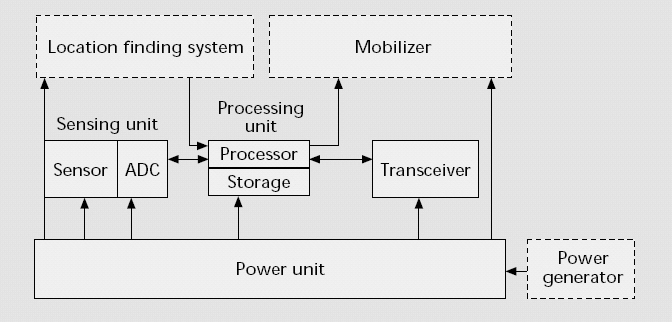
\includegraphics[width=8cm]{Componentes.jpg} 
\end{center}
\caption{Exemplo de imagem}
\label{fig:exemplo}
\end{figure} 

\section{Hip�teses Alternativas ao Enunciado}
A FAZER...

\section{Implementa��o}
C�digo em java

\subsection{Arquitectura do Sistema}
Multi Servidor
Multi Clientes por Servidor

\subsection{Estruturas de Dados}
Classes utilizadas
Estruturas de dados principais: PDU, ...
Servidor, Clientes, outras

\subsection{Bibliotecas Auxiliares}
A FAZER...????

\subsection{Outros Detalhes}
A FAZER...?????

\section{Testes e Resultados}
Snap shots e inputs de verbatim

\section{Conclus�o e Trabalho Futuro}


\section*{Acknowledgments}
O presente trabalho foi realizado no �mbito da unidade curricular de Comunica��es por Computador, 
ano lectivo de 2014/2015, da Licenciatura em Engenharia Inform�tica, da Universidade do Minho.

\bibliographystyle{splncs}
\bibliography{CC-2015-TP2-Grxx.tex}

\end{document}
